\documentclass[pscyr]{hedwork}
\usepackage[russian]{babel}
\usepackage{hedmaths}
\usepackage{graphicx}
\graphicspath{{images/}}

\usepackage{color}
\usepackage[colorlinks,linkcolor=black,urlcolor=black]{hyperref}
\renewcommand{\UrlFont}{\rm\small}

\newcommand{\Pic}[1]{\ref{pic#1}}
\newcommand{\pic}[1]{рис.~\Pic{#1}}

\faculty{Факультет электроники и вычислительной техники}
\department{экспериментальной физики}
\subject{дисциплине\\<<Методы и средства физического эксперимента>>}
\topic{Измерение сопротивлений косвенными методами}
\student[m]{студент группы Ф-469\\Чечеткин И. А.}
\teacher[m]{старший преподаватель\\Аршинов А. В.}

\geometry{left=2.5cm, top=2cm, bottom=2cm, right=1.5cm}

\begin{document}
  \maketitle
  \tableofcontents

  \section*{Введение}
  \addcontentsline{toc}{section}{Введение}
  
  Электрическое сопротивление~-- основная электрическая характеристика
  проводника, величина, характеризующая противодействие электрической цепи или
  ее участка электрическому току.

  Для практического измерения сопротивлений применяют множество различных
  методов, в зависимости от условий измерения и характера объектов, от требуемой
  точности и быстроты измерений. Например, различают методы для измерения
  сопротивления при постоянном токе и при переменном, методы измерения
  больших (свыше 1~МОм), средних (от 10~Ом до 1~МОм) и малых (меньше 10~Ом)
  сопротивлений, прямые и косвенные и~т.~д.

  \section{Измерение сопротивления при постоянном токе}

  Основными методами измерения сопротивления постоянному току являются косвенный
  метод, мостовой метод, компенсационные методы. Выбор метода измерений зависит
  от ожидаемого значения измеряемого сопротивления и требуемой точности
  измерений. Из косвенных методов наиболее универсальным является метод
  амперметра-вольтметра.

  \subsection{Метод амперметра-вольтметра}

  Данный метод основан на измерении тока, протекающего через измеряемое
  сопротивление и падения напряжения на нем. Применяют две схемы измерения:
  измерение больших сопротивлений (\pic{AV}а) и измерение малых сопротивлений
  (\pic{AV}б). По результатам измерения тока и напряжения определяют искомое
  сопротивление.
  
  \begin{figure}[!b]
    \center
    \includegraphics[width=.4\textwidth]{AVa} \hspace{2em}
    \includegraphics[width=.4\textwidth]{AVb} \\
    
    \vspace{-4em}
    \parbox{.4\textwidth}{\center а)} \hspace{2em}
    \parbox{.4\textwidth}{\center б)} \\
    \caption{Схемы измерения методом амперметра-вольтметра}
    \label{picAV}
  \end{figure}

  Для схемы (\pic{AV}а) искомое сопротивление можно определить по формуле:
  \[
    R_x \approx U / I_x.
  \]
  
  Для схемы (\pic{AV}б) искомое сопротивление определяются по формуле:
  \[
    R_x \approx U_x / I.
  \]
 
  Очевидно, что при подсчете искомого сопротивления по таким формулам возникает
  погрешность оттого, что при измерении токов и напряжений во второй схеме
  амперметр учитывает и тот ток, который проходит через вольтметр, а в первой
  схеме вольтметр измеряет напряжение помимо резистора еще и на амперметре.
  
  Для первой схемы сопротивление амперметра \( R_a \) будет являться абсолютной
  погрешностью измерений. Относительная же погрешность определяется следующим
  образом:
  \[
    \eps = \frac{R_x - R_t}{R_t} = \frac{R_a}{R_t} \approx \frac{R_a}{R_x},
  \]
  где \( R_t \) -- истинное значение измеряемого сопротивления. То есть точность
  измерения сопротивления будет тем больше, чем меньше сопротивление амперметра
  \( R_a \) по сравнению с измеряемым сопротивлением \( R_t \) (идеальным будет
  амперметр с бесконечно малым собственным сопротивлением).
  
  Для второй схемы абсолютная погрешность:
  \[
    \Delta R = \frac{R_x}{1 - R_x / R_v} - R_x = R_x \left( \frac{R_x / R_v}
      {1 - R_x / R_v} \right) = \frac{R_x^2}{R_v - R_x}.
  \]
  
  Относительная погрешность:
  \[
    \eps = \frac{\Delta R}{R_t} = \frac{R_x^2}{R_v - R_x} \cdot
      \frac{1 - R_x / R_v}{R_x} = \frac{R_x}{R_v}.
  \]
  Таким образом, точность измерения сопротивления будет тем больше, чем больше
  сопротивление вольтметра \( R_v \) по сравнению с измеряемым сопротивлением
  \( R_t \) (идеальным будет вольтметр с бесконечно большим собственным
  сопротивлением).

  Используемые при измерении приборы должны иметь класс точности не более 0,2.
  Вольтметр подключают непосредственно к измеряемому сопротивлению. Во избежание
  нагрева сопротивления и, соответственно, снижения точности измерений, ток в
  схеме измерения не должен превышать 20\% номинального.
  
  Достоинство схем метода амперметра-вольтметра заключается в том, что по
  резистору с измеряемым сопротивлением можно пропускать тот же ток, как и в
  условии его работы, что является важным при измерении сопротивлений, значения
  которых зависят от тока.
  
  \subsection{Мосты для измерения сопротивления на постоянном токе}
  
  \subsubsection{Одинарные мосты}  
  Для измерения сопротивления на постоянном токе широко используются одинарные 
  мосты. Одинарными мостами называют четырехплечие мосты с питанием от источника
  постоянного тока. Существует ряд конструкций этих приборов с различными
  характеристиками. Простейший~-- мост Уитстона. Погрешность моста зависит от
  пределов измерения и указывается обычно в паспорте моста.
  
  Конструктивно мосты оформляются в виде переносных приборов; они рассчитаны на
  работу с собственным или наружным нуль-индикатором. При измерении малых
  сопротивлений на результат измерения существенное влияние оказывают
  сопротивления контактов и соединительных проводов, суммируемые с измеряемым
  сопротивлением. Для уменьшения этого влияния используют специальные способы
  присоединения \( R_x \) к мосту, для чего мост имеет четыре зажима
  (\pic{sinbr}).
  
  \begin{figure}[!t]
    \center
    \includegraphics[width=.34\textwidth]{current_bridge} \hspace{2em}
    \includegraphics[width=.58\textwidth]{double_bridge} \\
    \parbox{.34\textwidth}{\caption{Одинарный мост} \label{picsinbr}}
      \hspace{2em}
    \parbox{.58\textwidth}{\caption{Двойной мост} \label{picdblbr}}
  \end{figure}

  При измерении сопротивлений от 10 Ом до 1 МОм зажимы 1 и 2, а также 3 и 4
  замыкаются перемычками и резистор с измеряемым сопротивлением подключается к
  зажимам 2 и 3 (I). Сопротивление \( R_x \) измеряется вместе с
  сопротивлением проводов и контактов, при помощи которых оно подключается к
  зажимам 2 и 3. При измерении малых сопротивлений (меньше 10 Ом) погрешность,
  вносимая соединительными проводами и контактами, может оказаться большой.
  Уменьшить её можно, подключив измеряемый резистор к 4 зажимам~-- 1 и 2, 3 и 4.
  При этом перемычки между точками 1 и 2, 3 и 4 снимаются, а точки А и 4, Б и 1
  соединяются между собой (II).

  В этом случае сопротивление провода от \( R_x \) к зажиму 2 входит в плечо
  сопротивлением \( R \), а сопротивление провода от \( R_x \) к зажиму 3~-- в
  плечо сопротивлением \( R_1 \). Сопротивления \( R \) и \( R_1 \) значительно
  больше сопротивлений проводов.

  Сопротивление \( R_x \) при равновесии моста (\( I_\text{НИ} = 0 \)):
  \[
    R_x = \frac{R R_1}{R_2}.
  \]
  
  Диапазон измерения: от 10~Ом до 0,1~ПОм%
    \footnote{\ \ 1 петаом = \( 10^{15} \) Ом}.
  
  Классы точности: от 0,005 до 10,0.

  При измерении весьма малых сопротивлений рассматриваемый мост имеет
  большие погрешности из-за низкой чувствительности. Повышение
  чувствительности увеличением тока питания ограничивается допустимой мощностью,
  рассеиваемой в плечах моста. Этого недостатка лишены двойные мосты.

  \subsubsection{Двойные мосты}

  Наиболее распространенной схемой, в которой влияние проводов и контактов
  сведено к минимуму, является схема двойного моста (\pic{dblbr}).
  
  Сопротивления плеч моста обозначены через \( R \) с соответствующими
  индексами, а сопротивления соединительных проводов и контактов через
  \( R_1' \), \( R_2' \) и т.д.
  
  Если принять сопротивления соединительных проводов и контактов входящими в
  значения сопротивлений, обозначенных буквами с соответствующими индексами, то
  при равновесии моста выполняются следующие условия:
  \begin{gather*}
    I_1 = I_2; \quad I_3 = I_4; \quad I_x = I_\text{н}; \\
    I_x R_x + I_3 R_3 = I_1 R_1; \\
    I_\text{н} R_\text{н} + I_4 R_4 = I_2 R_2; \\
    I_3 R_3 + I_4 R_4 = (I_x - I_3) R.
  \end{gather*}

  Решив эти уравнения относительно \( R_x \), найдем
  \[
    R_x = R_\text{н} \frac{R_1}{R_2} + \frac{R_4 R}{R + R_3 + R_4}
      \left( \frac{R_1}{R_2} - \frac{R_3}{R_4} \right).
  \]
  
  Из данного уравнения следует, что если выполнить условие
  \[
    \frac{R_1}{R_2} = \frac{R_3}{R_4},
  \]
  то второй член этого уравнения будет равен нулю и измеряемое сопротивление
  \( R_x \) можно определить из равенства:
  \[
    R_x = R_\text{н} \frac{R_1}{R_2}.
  \]

  Двойные мосты выполняются с постоянным или переменным отношением плеч.
  Гальванометр в момент равновесия может быть замкнут на небольшое
  сопротивление, поэтому при выборе гальванометра следует предпочесть приборы с
  малым внешним критическим сопротивлением и большей чувствительностью
  по напряжению. С целью расширения пределов измерения в промышленных приборах
  двойные мосты совмещаются с одинарными, обеспечивая широкие пределы измерений.
  
  Диапазон измерения: от 10~нОм до 10~Ом.
  
  Классы точности: от 0,01 до 2,0.
  
  \bigskip
  
  Существуют еще один класс мостов -- цифровые. Они рассчитаны на измерение
  очень больших сопротивлений и изготавливаются с использованием очень
  чувствительных средств измерения (одинарных мостов, баллистических
  гальванометров) и магазинов сопротивлений, измеренных с высокой точностью.
  
  Диапазон измерения: от 10~МОм до 1~ТОм, можно использовать для измерений до
    0,01~ЭОм\footnote{\ \ 1 эксаом = \( 10^{18} \) Ом}.
  
  Классы точности: от 0,005 до 2,0.
  
  \subsection{Компенсационный метод}
  
  В данном методе последовательно с измеряемым сопротивлением \( R_x \)
  включается образцовое сопротивление \( R_0 \) (\pic{comp}). Компенсационный
  метод имеет очень большую точность измерений.
  
  С помощью компенсатора (или вольтметра) измеряют падение напряжения на
  \( R_x \) и \( R_0 \), а так как сопротивления включены последовательно, то
  через них течет одинаковый ток и, следовательно,
  \[
    I_x = I_0 = I; \quad \frac{U_x}{R_x} = \frac{U_0}{R_0}; \quad
      R_x = R_0 \cdot \frac{U_x}{U_0}.
  \]
  
  \begin{figure}[!t]
    \center
    \includegraphics[width=.5\textwidth]{comp}
    \caption{Схема измерений компенсационным методом}
    \label{piccomp}
  \end{figure}

  \subsection{Измерение очень больших сопротивлений}
  
  Существует несколько методов измерения больших сопротивлений. Один из них~--
  метод непосредственного отклонения, в котором ток, протекающий через
  измеряемое сопротивление под воздействием известного напряжения,
  непосредственно определяется по чувствительному гальванометру, включенному
  последовательно с сопротивлением (\pic{AV}а). Напряжение на сопротивлении
  определяется по показанию включенного параллельно сопротивлению вольтметра.
  Величина искомого сопротивления находится на основании закона Ома делением
  напряжения на величину протекающего через него тока. Отличие этого метода от
  метода амперметра-вольтметра заключается лишь в замене амперметра на
  гальванометр с как можно большей чувствительностью.
  
  \bigskip

  Очень распространено измерение больших сопротивлений при помощи
  потенциометрических схем. Пределы измерений при этом могут быть значительно
  больше, а аппаратура надежнее и прочнее, чем при способе непосредственного
  отклонения. В большинстве промышленных мегомметров и тераомметров используется
  потенциометрический способ. Измеряемое \( R_x \) и образцовое \( R_0 \)
  сопротивления образуют делитель, питаемый от стабильного источника постоянного
  напряжения \( U \). Падение напряжения на образцовом сопротивлении измеряют
  вольтметром с высоким входным сопротивлением. При определенном значении
  напряжения \( U \) каждому показанию \( u \) вольтметра соответствует вполне
  определенное значение измеряемого сопротивления:
  \[
    R_x = (U - u) R_0 / u,
  \]
  и вольтметр отградуирован в единицах сопротивления.
  
  При осуществлении потенциометрического способа измерения возникают две
  проблемы: изготовления стабильного образцового сопротивления и выбора
  высокоомного и чувствительного вольтметра. Потенциометрические схемы
  различаются лишь по способу измерения напряжения на образцовом сопротивлении.

  \section{Измерение сопротивления при переменном токе}
  
  \subsection[Измеритель иммитанса]{Измеритель иммитанса (измеритель RLC)}
  
  Измерителем иммитанса, или измерителем \( RLC \), называют радиоизмерительный
  прибор, предназначенный для определения параметров полного сопротивления или
  полной проводимости электрической цепи.
  
  Среди основных методов измерения параметров электрических цепей можно назвать
  мостовые методы и метод, связанный с использованием соотношений закона Ома на
  переменном токе.
  
  Принцип действия мостовых измерителей иммитанса основан на использовании
  измерительного моста, для уравновешивания которого в приборе содержатся наборы
  образцовых активных и реактивных сопротивлений. Такие приборы могут работать
  только на фиксированных частотах. Реализация цифровых приборов для измерения
  параметров электрических цепей на основе мостовых методов сопровождается
  заметным усложнением их схемотехники и автоматизации процессов уравновешивания.
  
  Приборы, в основу которых положено использование соотношений закона Ома,
  проще с точки зрения схемотехнической реализации и автоматизированного
  получения результата измерения. Принцип измерения таких измерителей иммитанса
  основан на анализе прохождения тестового сигнала (обычно синусоидального) с
  заданной частотой через измеряемую цепь, обладающую комплексным
  сопротивлением. Напряжение рабочей частоты с внутреннего генератора подается
  на измеряемый объект. На выделенном участке цепи измеряется напряжение, ток и
  фазовый сдвиг между ними. Измеренные величины используются для расчёта
  параметров цепей.
  
  Мостовые схемы и схемы для измерения сопротивления с использованием
  соотношений закона Ома на переменном токе такие же, как и схемы на постоянном
  токе (\pic{AV}, \pic{sinbr}, \pic{dblbr}), с точностью до замены обычного
  сопротивления на комплексное.
  
  \subsection{Измерительная линия}

  Измерительная линия~-- это устройство для исследования распределения
  электрического поля вдоль СВЧ-линии передачи. Измерительная линия представляет
  собой отрезок коаксиальной линии или волновода с перемещающимся вдоль него
  индикатором, отмечающим узлы (пучности) электрического поля. С помощью
  измерительной линии исследуется распределение напряженности электромагнитного
  поля, из которого определяются коэффициент стоячей волны как отношение
  амплитуд волны в пучности и узле и фаза коэффициента отражения по смещению
  узла. Зная эти параметры, по круговой диаграмме полных сопротивлений можно
  найти полное сопротивление. Измерения производятся с использованием
  измерительного генератора в качестве источника сигнала. Для отсчета показаний
  используются, как правило, гальванометр или измеритель отношений напряжений.
  Измерительные линии применяются на частотах от сотен мегагерц до сотен
  гигагерц.

  \begin{figure}[!t]
    \center
    \includegraphics{line}
    \caption{Общая схема измерительной линии}
    \label{picline}
    { \small
      З~-- зонд; ИГ~-- индикаторная головка (каретка); Д~-- детектор; И~--
      индикатор; Ш~-- шкала отсчёта перемещения ИГ; Г~-- генератор СВЧ; А~--
      аттенюатор; \( Z_\text{н} \)~-- нагрузка.
    }
  \end{figure}

  Линия состоит из трех основных узлов (\pic{line}): отрезка передающей линии с
  продольной узкой щелью, зондовой головки и каретки с механизмом для
  перемещения зондовой головки вдоль линии. Зондовая головка представляет собой
  резонатор, возбуждаемый зондом~-- тонкой проволокой, погруженной через щель во
  внутреннюю полость волновода. Глубину погружения зонда в линии регулируют
  специальным винтом, расположенным сверху зондовой головки. Внутри резонатора
  помещен полупроводниковый детектор, связанный с индикаторным прибором. При
  перемещении зонда вдоль линии, внутри которой имеется электромагнитное поле,
  в зонде наводится электродвижущая сила, пропорциональная напряженности поля в
  сечении расположения зонда. Эта ЭДС возбуждает резонатор, создавая в нем
  электромагнитные колебания. Для уменьшения искажающего действия зонда на
  электромагнитное поле в линии и повышения чувствительности линии объемный
  резонатор зондовой головки настраивают в резонанс с частотой электромагнитных
  колебаний.
  
  \bigskip

  Для измерения полного сопротивления цепи также используется устройство,
  называемое измерителем полных сопротивлений. Измерители полного сопротивления
  имеют меньшую чувствительность, чем измерительные линии, однако они имеют
  существенно меньшие размеры, особенно в нижней части диапазона частот.
  Коэффициент стоячей волны, как и в измерительных линиях, определяется из
  отношения показаний низкочастотного индикатора при экстремальных значениях
  сигнала. Импеданс исследуемого объекта находят по круговой диаграмме полных
  сопротивлений исходя из значений коэффициента стоячей волны и фазы
  коэффициента отражения.

  \section{Измерение ультрамалых сопротивлений}

  В профессиональной и радиолюбительской практике приходится встречаться с
  необходимостью измерения ультрамалого сопротивления. К числу задач, требующих
  измерения сопротивлений вплоть до 1~мОм с заданной точностью, относятся,
  например, изготовление шунтов (в том числе и для измерительных приборов),
  измерение переходного сопротивления контактов реле, переключателей и т.~п.
  Аналогичная задача возникает и при необходимости отбора мощных полевых
  транзисторов.
  
  В широко распространенных методах измерения последовательно с измеряемым
  сопротивлением \( R_x \) неизбежно включено паразитное сопротивление
  \( R_\text{п} \), образованное соединительными проводами, переходным
  сопротивлением входных клемм или гнезд, контактных переключателей и т.~п.
  Ввиду того что сопротивление \( R_\text{п} \) включено последовательно с
  \( R_x \), омметр измеряет их суммарное значение. Конечно, для больш\'{и}х
  значений сопротивления эта ошибка невелика и ее не учитывают. Иначе обстоит
  дело при измерении малых значений. Несложно заметить, что для значений
  \( R_x \) соизмеримых с сопротивлением \( R_\text{п} \), измерение в принципе
  еще возможно, хотя о точности говорить уже не приходится. Это действительно
  так для обычных, применяемых в аналоговых и цифровых омметрах, методов
  измерения сопротивления. Тем не менее эта задача давно успешно решена в более
  сложных приборах для измерения малых значений сопротивления методом амперметра
  и милливольтметра (\pic{ultra}).
  
  \begin{figure}[!t]
    \center
    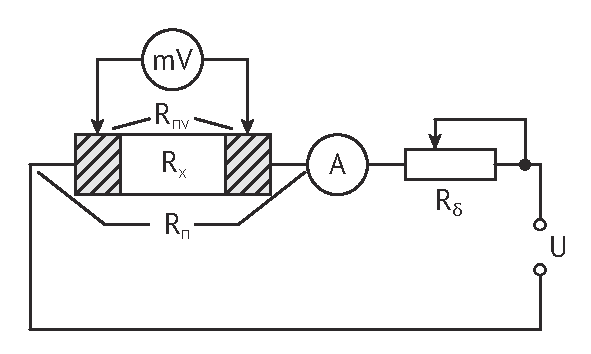
\includegraphics[width=.6\textwidth]{ultra}
    \caption{Схема измерения ультрамалых сопротивлений}
    \label{picultra}
  \end{figure}
 
  Через измеряемое сопротивление \( R_x \) пропускают ток, регулируемый
  балластным резистором \( R_\delta \) и контролируемый амперметром. Падение
  напряжения на \( R_x \) измеряют милливольтметром. Вольтметр подключен
  непосредственно к \( R_x \), поэтому влияние \( R_\text{п} \) полностью
  исключается. При этом, правда, появляется паразитное сопротивление
  \( R_\text{пv} \) в цепи вольтметра, образуемое контактным сопротивлением в
  точках подключения вольтметра (на рисунке показаны стрелками) и сопротивлением
  соединительных проводов вольтметра. Однако влияние \( R_\text{пv} \)
  пренебрежимо мало и его можно не учитывать, поскольку условие
  \( R_v > R_\text{пv} \) (где \( R_v \)~-- входное сопротивление вольтметра)
  выполняется практически всегда (минимальное значение входного сопротивления
  мультиметра у самых простых моделей составляет 1~МОм, а значение
  \( R_\text{пv} \) гораздо меньше 1~кОм). Значение \( R_x \) измеряемого
  сопротивления вычисляют по известной простейшей формуле
  \[
    R_x = U / I.
  \]

  \pagebreak

  \begin{thebibliography}{9}
  \addcontentsline{toc}{section}{Список литературы}
    \bibitem{1} Раннев,~Г.~Г. Методы и средства измерений: Учебник для вузов~/
      Г.~Г.~Раннев, А.~П.~Тарасенко~-- М.:~Издательский центр <<Академия>>,
      2004.~-- 336~с.
    \bibitem{2} Грибанов,~Ю.~И. Измерение слабых токов, зарядов и больших
      сопротивлений~/ Ю.~И.~Грибанов~-- Л.: Госэнергоиздат, 1962.
    \bibitem{3} Электрические измерения: Учебник для вузов~/ Байда~Л.~И.,
      Добротворский~Н.~С. и~др. Под ред. А.~В.~Фремке и Е.~М.~Душина~--
      5-е~изд., перераб. и доп.~-- Л.: Энергия. Ленинрадское отделение, 1980.
    \bibitem{4} Измерение сопротивления постоянному току. Режим доступа:\\
      \url{http://www.sonel.ru/ru/biblio/article/resistance-directcurrent/}\\
      (дата обращения 20.11.2013).
    \bibitem{5} Измерение ультрамалых сопротивлений. Режим доступа:\\
      \url{http://radioradar.net/articles/technics_measurements/%
      measurements_ultra.html}\\
      (дата обращения 20.11.2013).
    \bibitem{6} Погрешности измерения сопротивлений. Режим доступа:\\
      \url{http://edu.dvgups.ru/metdoc/enf/phizik/phizik/%
      lab_rab/lr_elect/povx/mu1.htm}\\
      (дата обращения 20.11.2013).
  \end{thebibliography}
\end{document}
